% Auto-generated by make_accuracy_figs.py — paste into your report.
% Figures are vector PDFs in accuracy_figs/.

\begin{figure}[htbp]
  \centering
  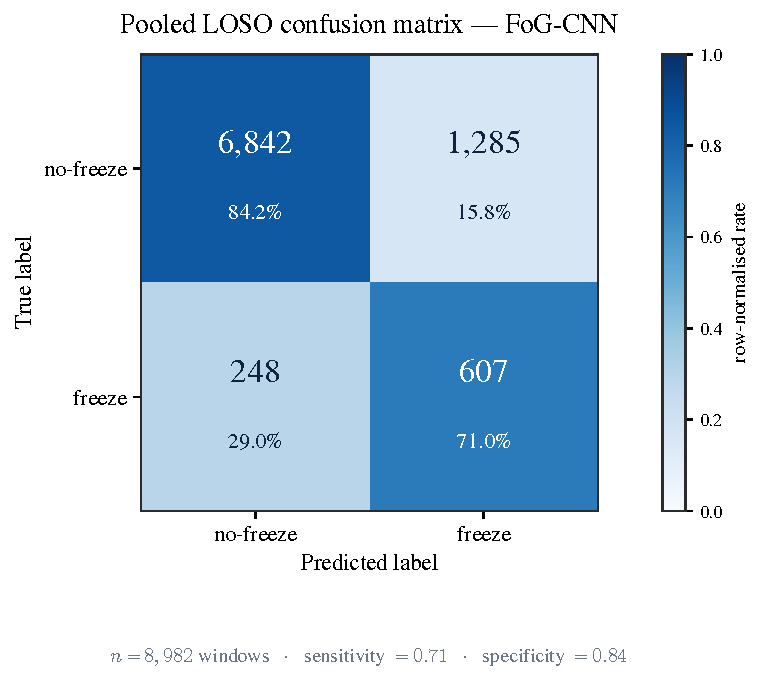
\includegraphics[width=0.8\linewidth]{accuracy_figs/confusion_matrix.pdf}
  \caption{Pooled leave-one-subject-out confusion matrix for the FoG-CNN (counts and row-normalised rates).}
  \label{fig:confusion_matrix}
\end{figure}

\begin{figure}[htbp]
  \centering
  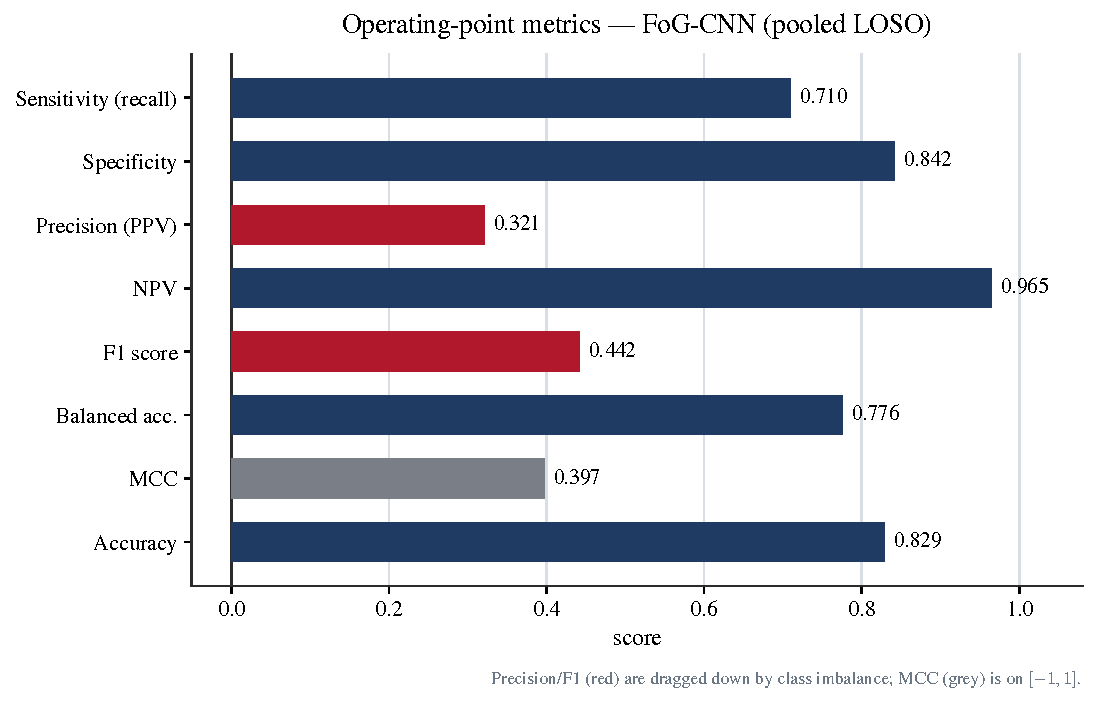
\includegraphics[width=0.8\linewidth]{accuracy_figs/metrics_panel.pdf}
  \caption{Operating-point metrics derived from the pooled LOSO confusion matrix.}
  \label{fig:metrics_panel}
\end{figure}

\begin{figure}[htbp]
  \centering
  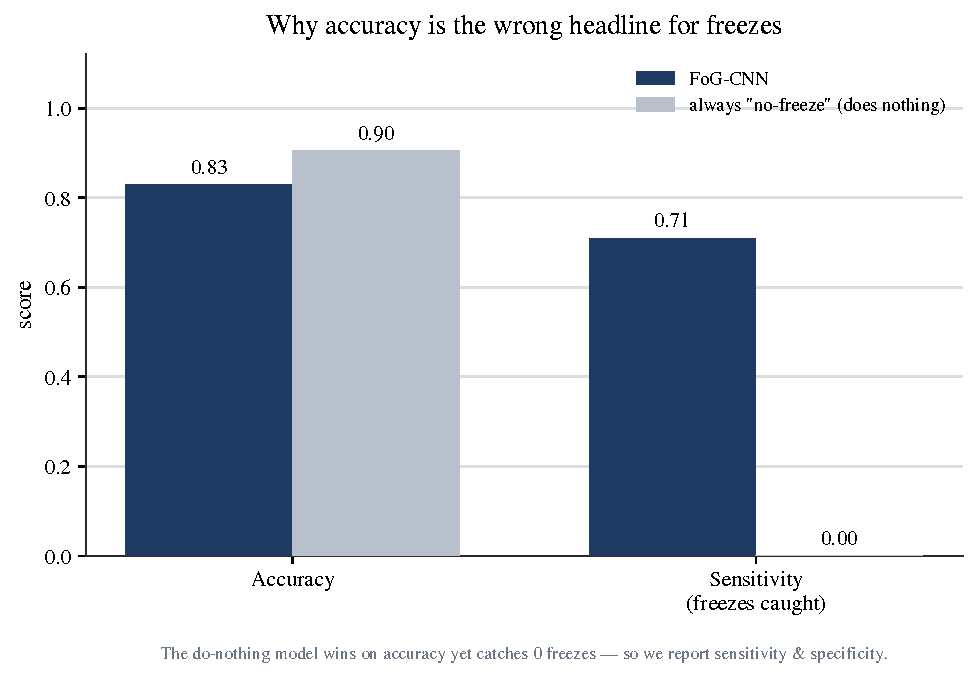
\includegraphics[width=0.8\linewidth]{accuracy_figs/accuracy_caveat.pdf}
  \caption{Accuracy is misleading under class imbalance: a do-nothing classifier beats the CNN on accuracy while detecting no freezes.}
  \label{fig:accuracy_caveat}
\end{figure}

\begin{figure}[htbp]
  \centering
  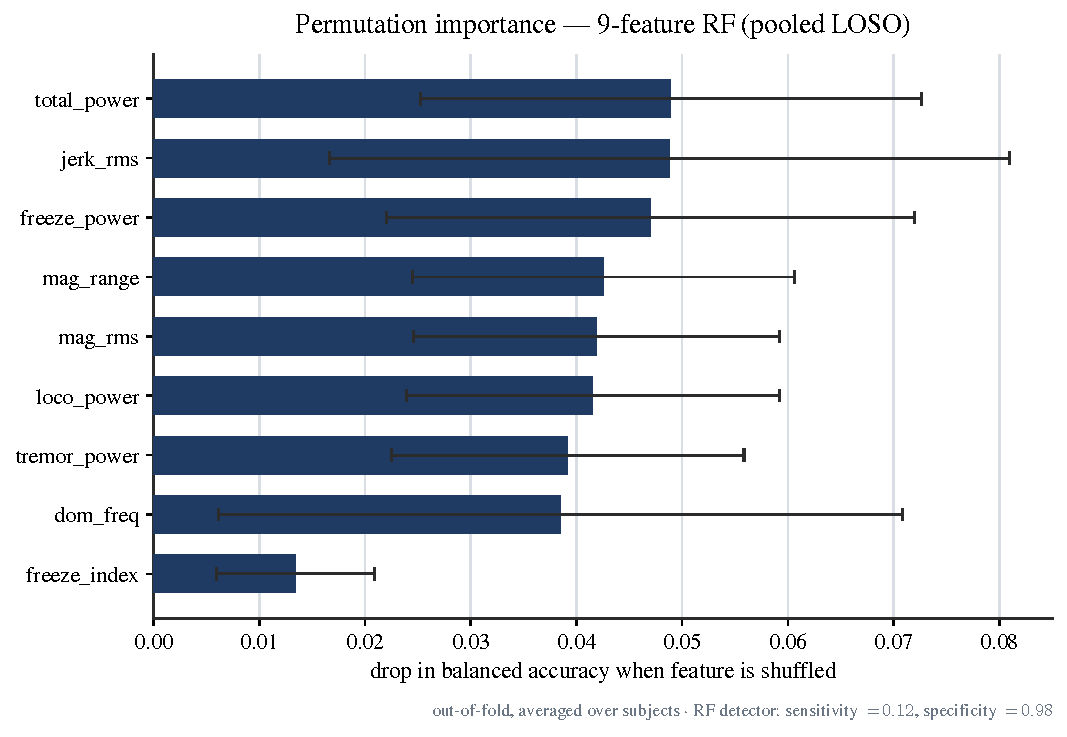
\includegraphics[width=0.8\linewidth]{accuracy_figs/perm_importance.pdf}
  \caption{Permutation importance of the nine engineered features for the interpretable RandomForest, aggregated out-of-fold over all pooled leave-one-subject-out folds (mean $\pm$ s.d. of the drop in balanced accuracy when each feature is shuffled).}
  \label{fig:perm_importance}
\end{figure}

\begin{figure}[htbp]
  \centering
  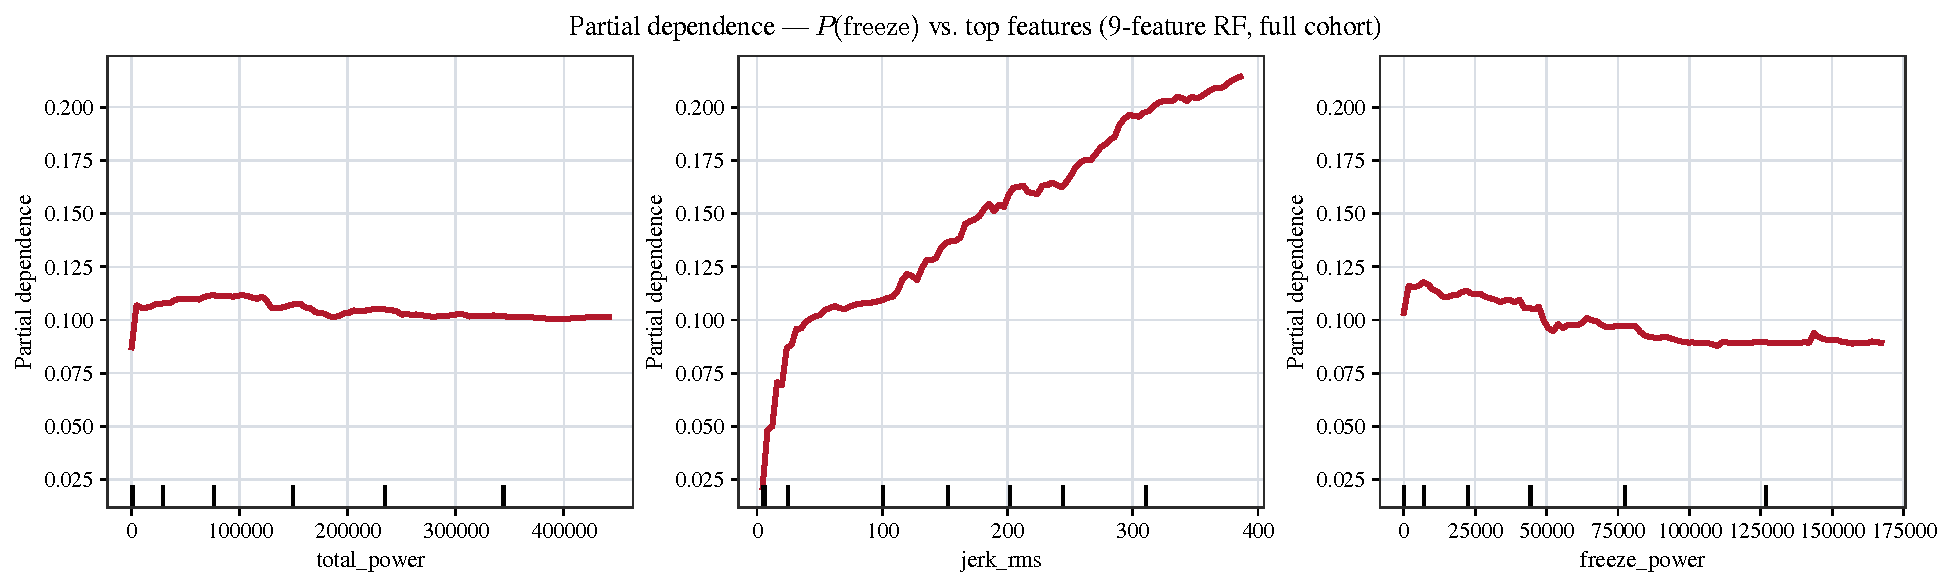
\includegraphics[width=0.8\linewidth]{accuracy_figs/partial_dependence.pdf}
  \caption{Partial dependence of $P(\mathrm{freeze})$ on the three most important features for the 9-feature RandomForest (fit on the full cohort).}
  \label{fig:partial_dependence}
\end{figure}

\begin{figure}[htbp]
  \centering
  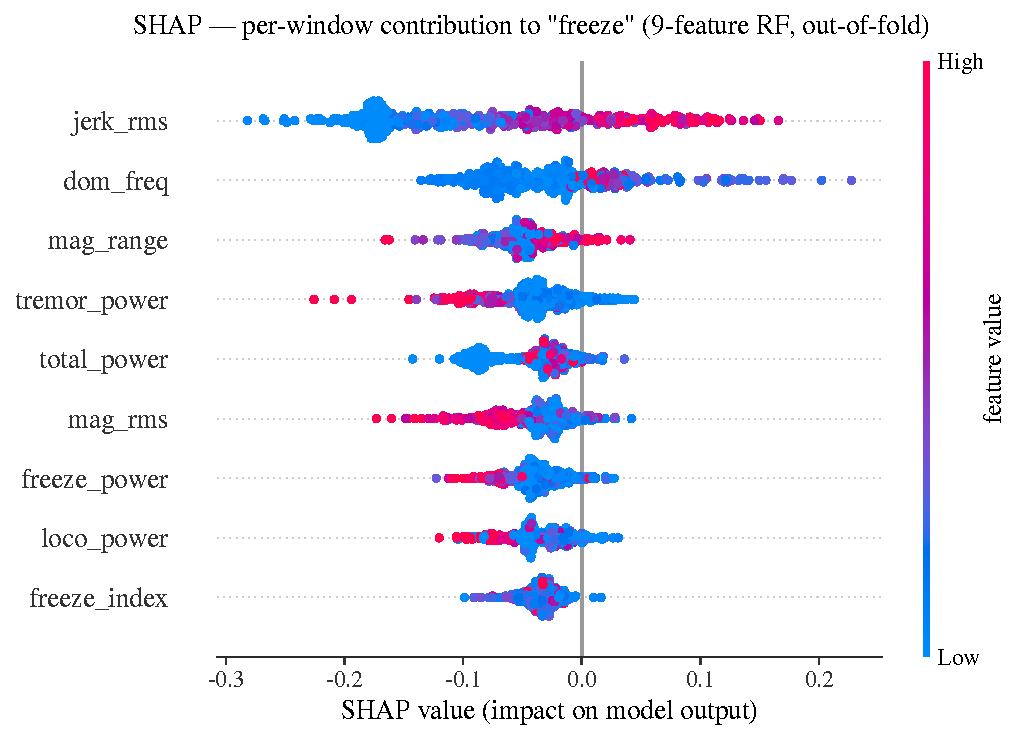
\includegraphics[width=0.8\linewidth]{accuracy_figs/shap_beeswarm.pdf}
  \caption{SHAP values for the 9-feature RandomForest: per-window, out-of-fold contribution of each feature to the ``freeze'' prediction.}
  \label{fig:shap_beeswarm}
\end{figure}

\begin{figure}[htbp]
  \centering
  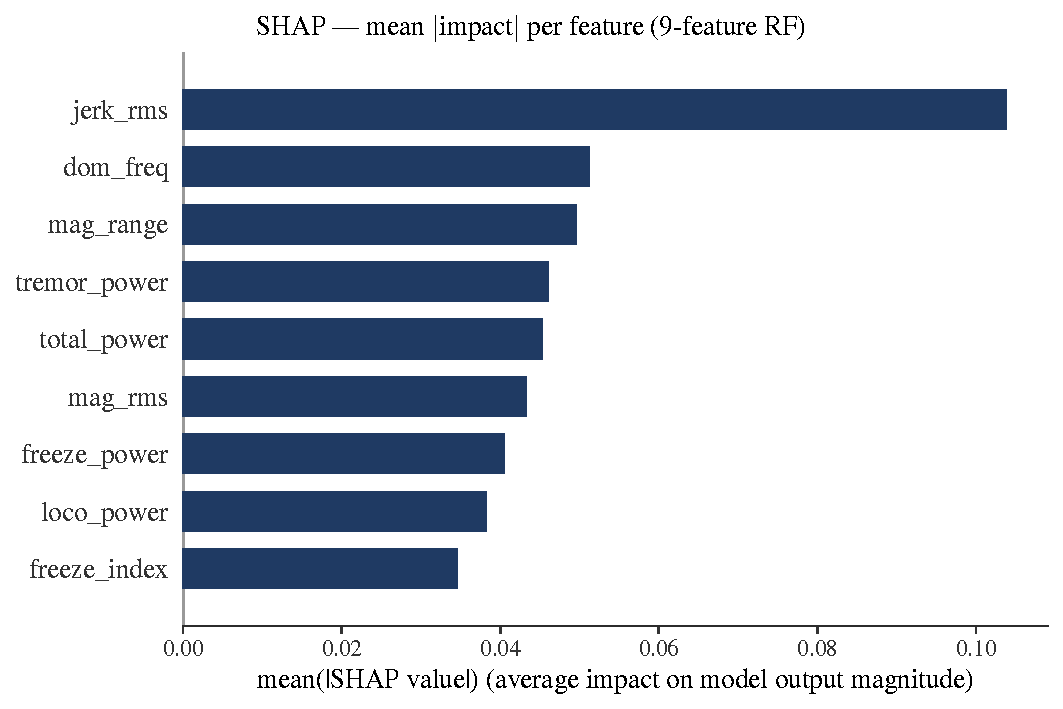
\includegraphics[width=0.8\linewidth]{accuracy_figs/shap_bar.pdf}
  \caption{Mean absolute SHAP value per feature for the 9-feature RandomForest.}
  \label{fig:shap_bar}
\end{figure}

\begin{figure}[htbp]
  \centering
  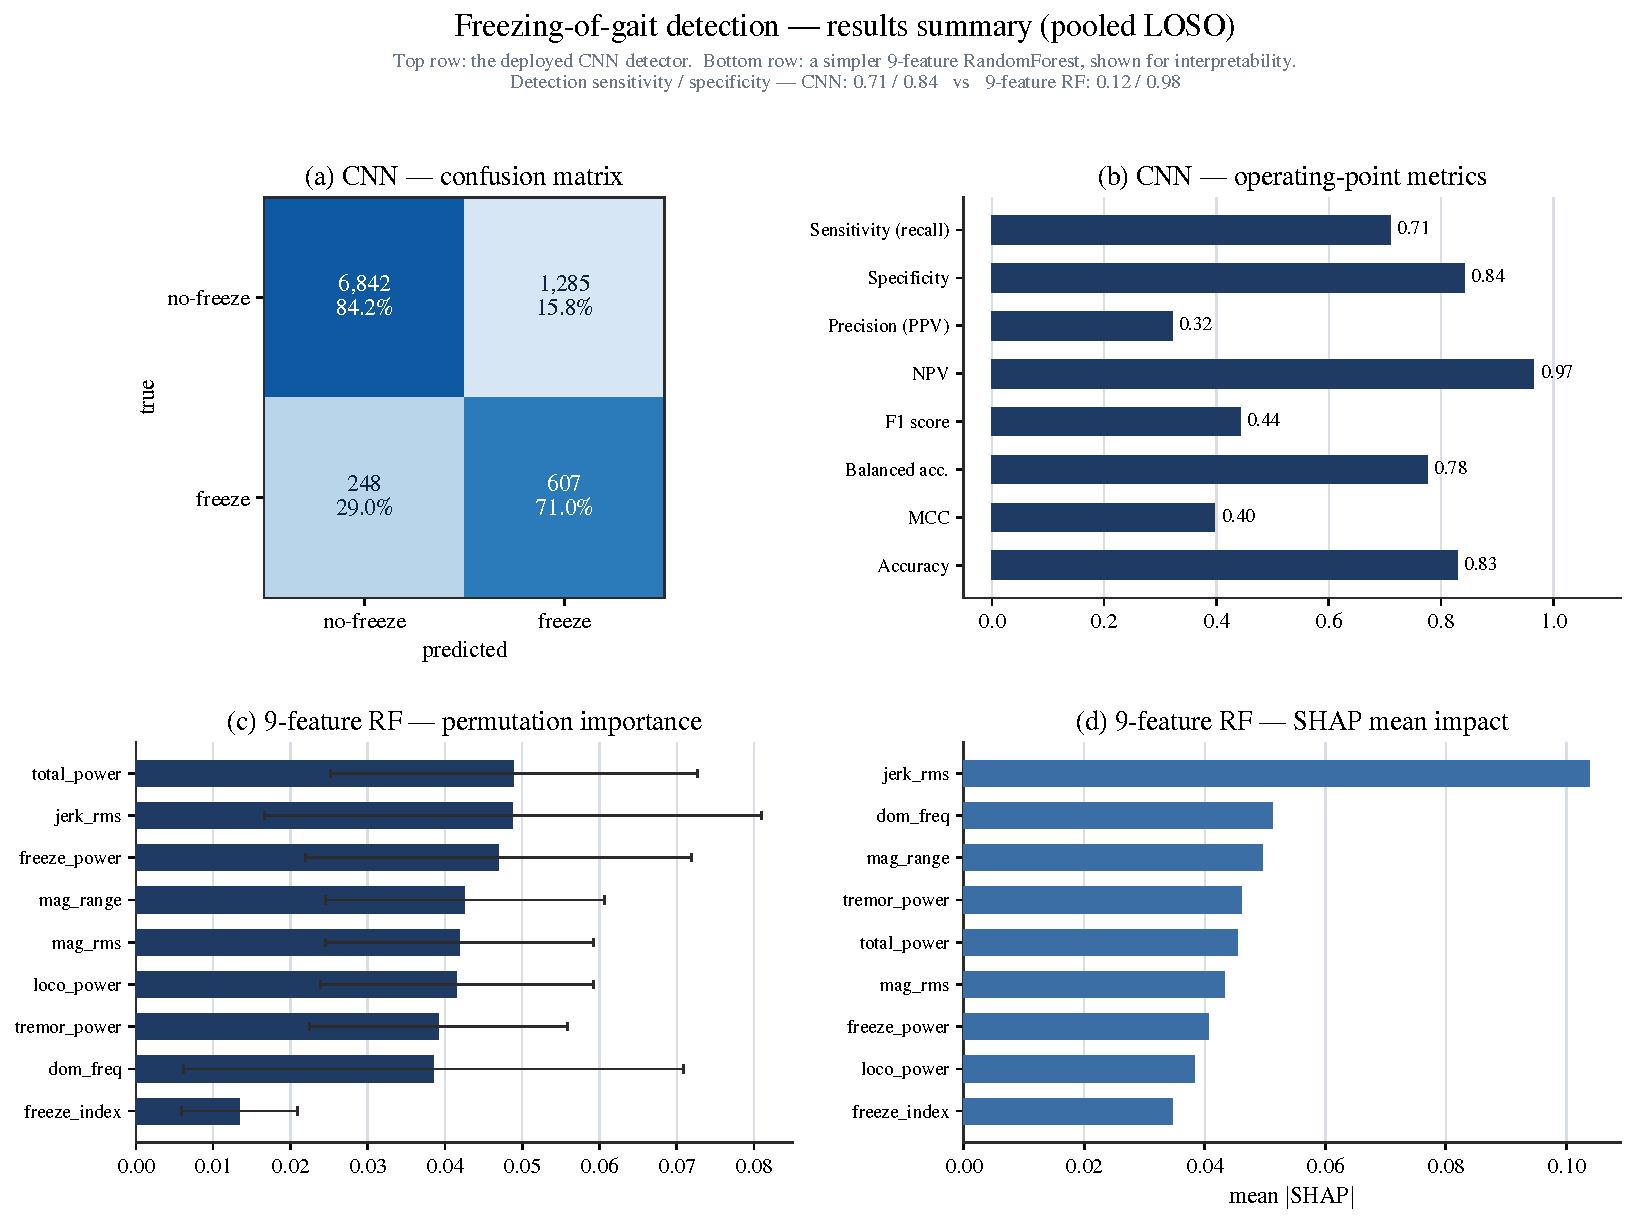
\includegraphics[width=0.8\linewidth]{accuracy_figs/results_sheet.pdf}
  \caption{One-page results summary: the deployed CNN (confusion matrix and operating-point metrics, panels a--b) alongside the interpretable 9-feature RandomForest (permutation importance and SHAP, panels c--d), all under pooled leave-one-subject-out.}
  \label{fig:results_sheet}
\end{figure}
